% vim:set ft=tex:
\section{Fiasco.OC \& L4Re}
\label{state:env}
\todo{Fiasco.OC \& L4Re}

\textbf{Fiasco.OC}
\begin{itemize}
  \item Kernel scheduler does no balancing, assigns thread to the first
    core specified in the affinity descriptor
  \item affinity descriptor: core(s) a thread should run on
  \item Syscall via run\_thread() to pass affinity descr to kernel scheduler
  \item interface to query execution time for each thread
  \item capability system -- to derive communication relationships from
  \item	Kernel feature wishes derived from related work: Performance counters
    and per thread accounting
\end{itemize}

\textbf{L4Re}
\begin{itemize}
  \item provides scheduler proxy interface, including affinity descriptor,
    scheduling parameters
  \item syscall interface
\end{itemize}


% -----------------------------------------------------------------------------

\section{\gls{intel} Haswell Architecture}
\label{state:haswell}

In section \ref{state:related} several hardware features were mentioned.
The most important of all are performance counters for cache misses, cycles and
instructions executed.
Those and many more are present in the target processor: an \gls{intel} Core
i7-6440K.
The processor has ``architectural performance monitoring version 3''
capabilities, which consists among other features of three fixed-function
performance counters counting Instruction Retired, Unhalted Core Cycles, and
Reference Instruction Retired.
In contrast to the first two counters, the last counter is unaffected by
processor speed changes due to power saving or turbo boost features.
Besides these, four general purpose performance counters are available per
logical core, which can be programmed to count one specific event.
All \gls{intel} Core i generations support architectural performance monitoring
in different versions, but all versions are guaranteed to support the events
listed in table \ref{state:table:core_events}: Unhalted Core Cycles,
Instruction Retired, Unhalted Reference Cycles, LLC Reference, LLC Misses,
Branch Instruction Retired, and Branch Misses Retired.

Besides these central events, each hardware generation supports a different set
of so called ``non-architectural performance events''.
This non-architectural event set allows to monitor many specific events, e.g.
L2-misses/-hits, micro-ops per logical core executed per cycle, or unhalted
core cycles, while the logical core is in ring 0.

Another difference to the target processor, compared to most processors used in
earlier research is the \gls{smp} architecture. In contrast to \gls{cmp}
architectures no cache groups are defined by the hardware, because the
\gls{llc} is shared among all cores.
Figure \ref{state:fig:core_layout} shows examplary the cache hierarchy and core
components of the \gls{intel} Haswell processor.
Each core consists of two \gls{ht} cores, sharing L1- and L2-caches.
Besides the \gls{llc} the cores on one socket share nothing.
The caches are inclusive, meaning each cache line present in L1I or L1D
cache is also present in the corresponding L2 cache and each L2 cache line is
also present in the \gls{llc}.
This eases the lookup of cache lines in other cores on the same package.

%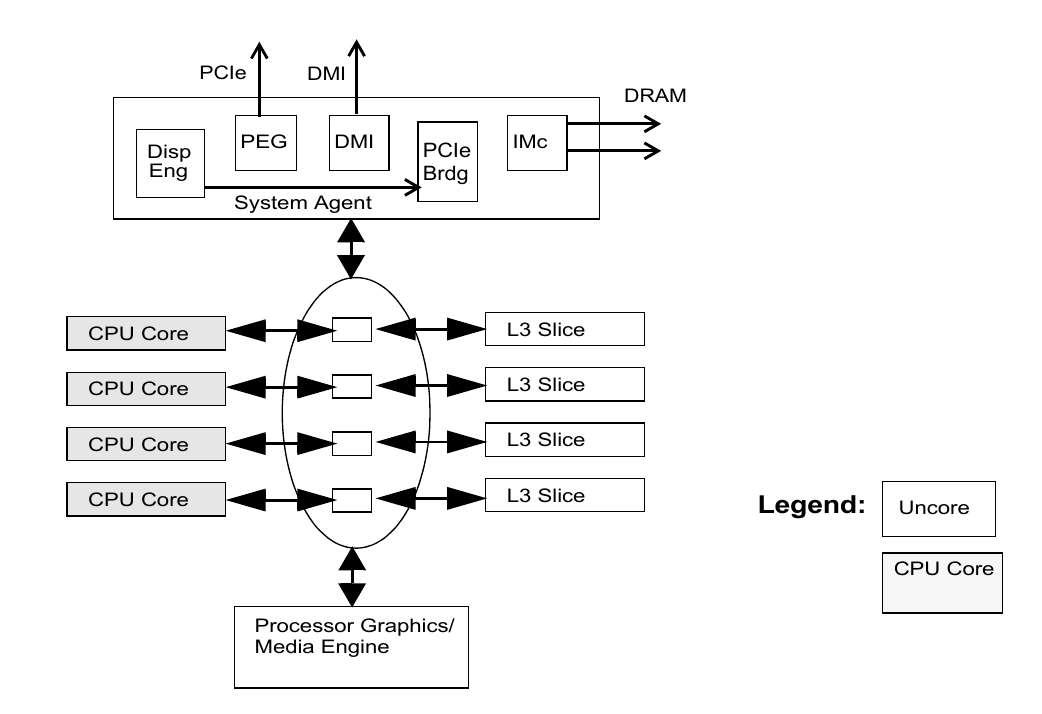
\includegraphics[width=0.8\textwidth]{images/haswell_architecture_by_intel_large}

\begin{figure}[h!]
  \centering
  \includegraphics[width=0.7\textwidth]{images/haswell_core_layout}
  \caption{Layout of a Core i7-4660K quad-core.
    Each physical core has two logical cores T0 and T1 sharing the cores L1I-,
    L1D-, and L2-cache.}
  \label{state:fig:core_layout}
\end{figure}


\begin{itemize}
  \item diagram of architecture: four cores with L1I/D \& L2 cache; two smt/ht
    cores per physical core; L3 cache shared and sliced, ring buffer for
    access; mem controler in uncore package;
  \item 4 prefetcher per cache; 2 for L1D, 2 for L2 cache
  \item L1D \& L2 cache data is present in L3 cache to be able to redirect
    requests from other cores to the correct cache. --> Issue with security; no
    cache side attack surface reduction
  \item IF security: dual socket system with one core dedicated to security
    tasks for an interval
  \item L3 cache slices corespond to number of cores
  \item logic portion and data array portion; access, coherency, memory
    ordering, LLC misses, writeback to memory; cache lines
  \item hash function uniformly distributes addresses
  \item access times to L3 cache varies depending on travel distance on the
    bi-directional ring buffer
  \item system agent receives memory requests not serviced by cache and
    redirects to IMC
\end{itemize}

\paragraph{Issues with security core idea:}
The idea to reduce attack surface for e.g. openssh cache attacks was to provide
a dedicated core for security critical applications.
This idea spawned from the assumption that L1D \& L2 cache was solely present
on a core, but the L3 cache content is a superset of all cores L1D \& L2 cache.
Hence, cache side channel attacks are still possible, although more
complicated, as the attacker not present on the core, must determine, which
cache lines correspond to the L1D \& L2 cache of the ``security core''.
Attacks presented in \cite{yarom_recovering_2014} and
\cite{bernstein_cache-timing_2005} rely on the fact, that only one application
is using cache lines on the core.
On a multicore, only observing the \gls{llc}, other running applications are
expected to disturb the observations, effectivly reducing the side channel
throughput.
\todo{This should be part of the architecture chapter, as the security core
idea wasn't presented yet.}

% -----------------------------------------------------------------------------
